%%%%%%%%%%%%%%%%%%%%%%%%%%%%%%%%%%%%%%%%%%%%%%%%%%%%%%%%%%%
\section{Равенство векторов}
%%%%%%%%%%%%%%%%%%%%%%%%%%%%%%%%%%%%%%%%%%%%%%%%%%%%%%%%%%%
Ненулевые векторы называются \textbf{коллинеарными}, если они лежат или на одной прямой,
или на параллельных прямых. Нулевой вектор считается коллинеарным любому вектору.

На рисунке векторы $\vv{a}$, $\vv{b}$, $\vv{c}$ и $\vv{d}$ коллинеарны, а
вектор $\vv{e}$ не коллинеарен ни одному из векторов.

Если два ненулевых вектора коллинеарны, то они могут быть направлены или одинаково,
или противоположно. В первом случае векторы называются \textbf{сонаправленными}, а во втором
\bdash \textbf{противоположно направленными}.

На рисунке~\ref{pic:vec_coll} векторы $\vv{a}$ и $\vv{b}$
сонаправлены ($\vv{a}\uparrow\uparrow\vv{b}$),
а векторы $\vv{c}$ и $\vv{d}$ противоположно направлены ($\vv{c}\uparrow\downarrow\vv{d}$).

Векторы называются \textbf{противоположными}, если они противоположно направлены и их длины равны.
Вектор, противоположный вектору $\vv{a}$ обозначается $-\vv{a}$.

Векторы называются \textbf{равными}, если они сонаправлены и их длины равны.

Таким образом, векторы $\vv{a}$ и $\vv{b}$ равны, если $\vv{a}\uparrow\uparrow\vv{b}$
и $|\vv{a}|=|\vv{b}|$. Равенство векторов обозначается так: $\vv{a}=\vv{b}$.

\begin{figure}[h]
  \centering
  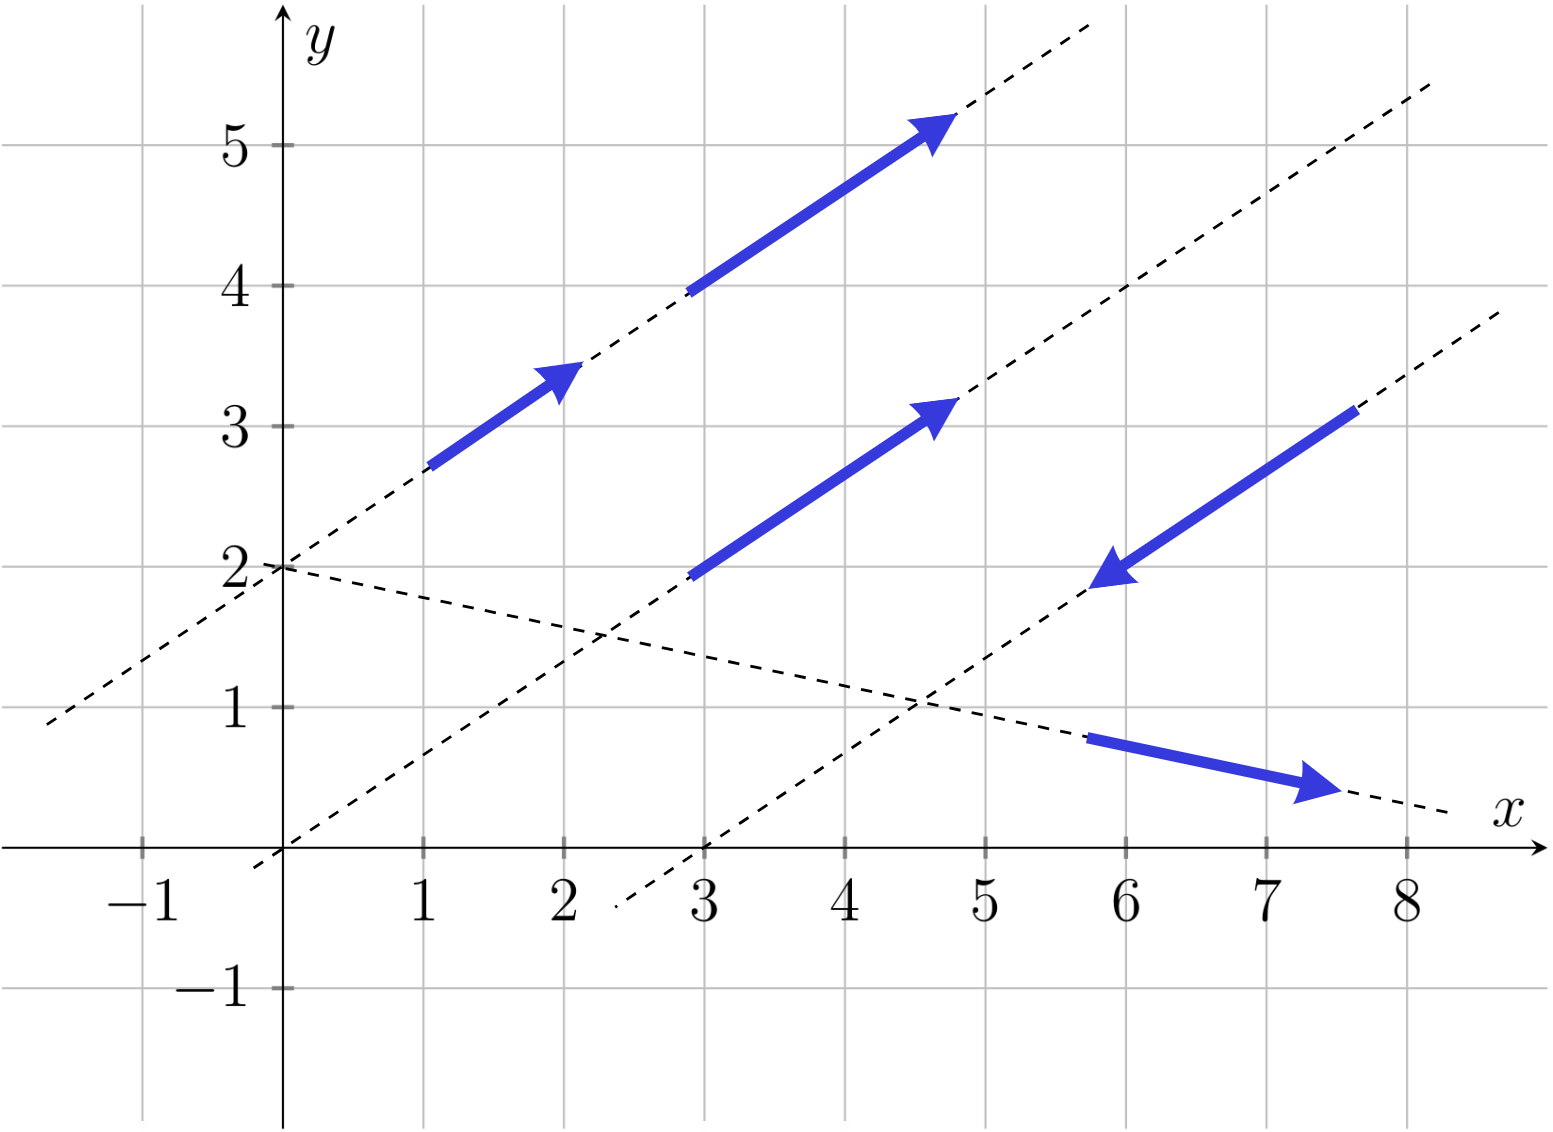
\includegraphics[width=0.7\textwidth]{pics/axis_l.png}
  \put(-180,215){\large $\vv{a}$}
  \put(-250,170){\large $\vv{c}$}
  \put(-180,150){\large $\vv{b}$}
  \put(-90,150){\large $\vv{d}$}
  \put(-80,90){\large $\vv{e}$}
  \caption{\small Коллинеарные и неколлинеарные векторы.}\label{pic:vec_coll}
\end{figure}

\clearpage

Если точка $A$ \bdash начало вектора $\vv{a}$, то говорят, что вектор $\vv{a}$
\textbf{отложен от точки} $A$. Верно следующее утверждение: от любой точки $M$ можно отложить
вектор, равный данному, и при том только один.

Равные векторы, отложенные от разных точек, часто обозначают одной и той же буквой.
Иногда говорят, что это один и тот же вектор, отложенный от разных точек.

%\begin{center}
%  \begin{tikzpicture}
%    \begin{axis}[
%        axis lines=middle,
%        axis equal image,
%        grid=major,
%        xmin=-2,
%        xmax=9,
%        ymin=-2,
%        ymax=6,
%        xlabel=$x$,
%        ylabel=$y$,
%        xtick={-1,...,8},
 %       ytick={-1,...,5},
%        tick style={thick},
%        width=12cm
%      ]
%    \end{axis}
%    \coordinate (A) at (3cm,5cm);
%    \coordinate (B) at (6cm,8cm);
%    %\draw [-latex, thick] (A) -- (B);
%    %\draw (1.2cm,1.3cm) node {$\vv{a}$};
%    \coordinate (C) at (0cm,0cm);
%    \coordinate (D) at (3cm,2cm);
%    \coordinate (E) at (0cm,0cm);
 %   \coordinate (F) at (3cm,2cm);
%    \coordinate (G) at (0cm,0cm);
%    \coordinate (H) at (3cm,2cm);
%    
%  \end{tikzpicture}
%\end{center}

Рисунок~\ref{pic:auto} иллюстрирует направление скоростей автомобилей,
когда их скорости сонаправлены, противоположно направлены, равны и противоположны.

\begin{figure}[h]
  \centering
  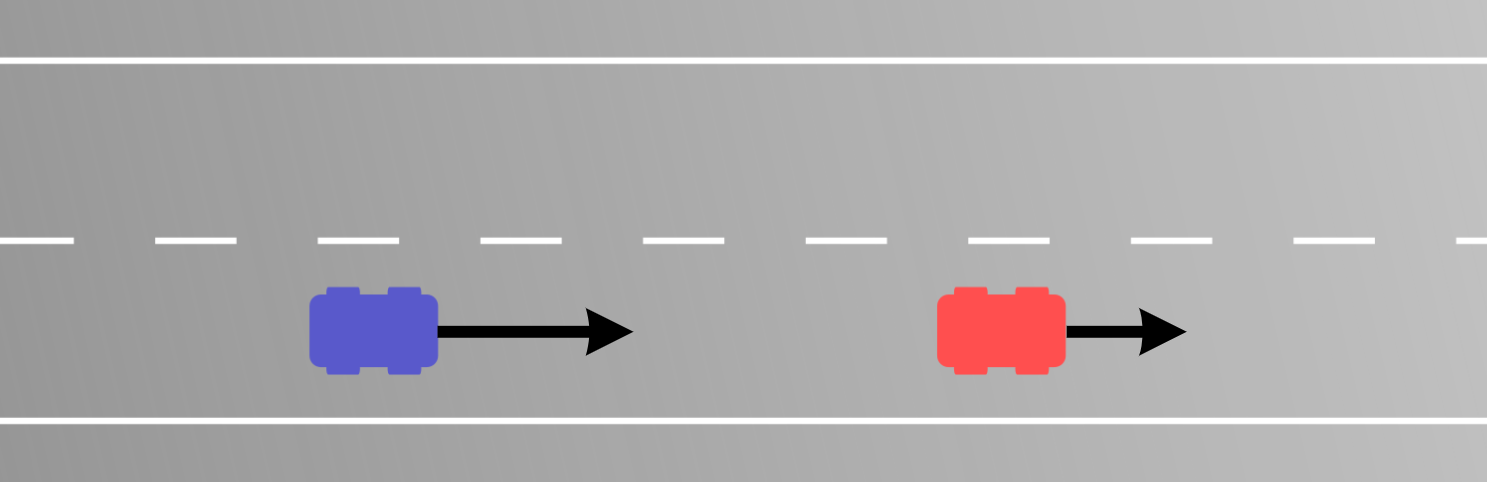
\includegraphics[width=0.48\textwidth]{pics/auto1.png}
  \put(-155,33){\large $\vv{v_1}$}
  \put(-65,33){\large $\vv{v_2}$}
  \put(-200,88){скорости сонаправлены $\vv{v_1}\uparrow\uparrow\vv{v_2}$}\hspace*{7mm}
  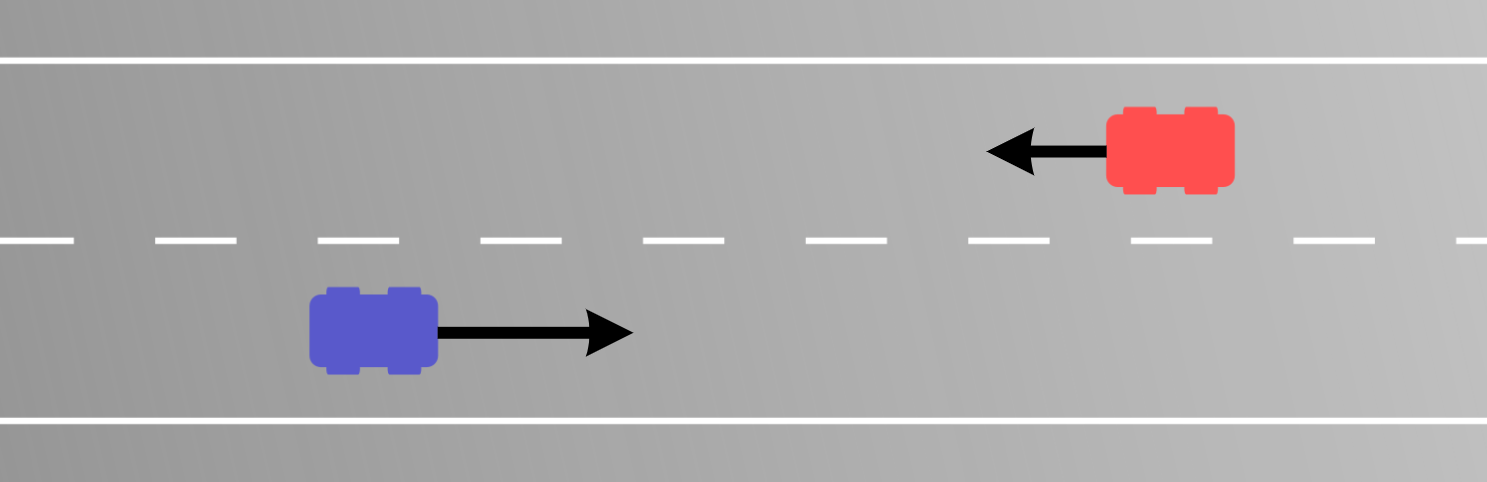
\includegraphics[width=0.48\textwidth]{pics/auto4.png}
  \put(-155,33){\large $\vv{v_1}$}
  \put(-75,65){\large $\vv{v_2}$}
  \put(-245,88){скорости противоположно направлены $\vv{v_1}\uparrow\downarrow\vv{v_2}$}
  \vspace{5mm}
  
  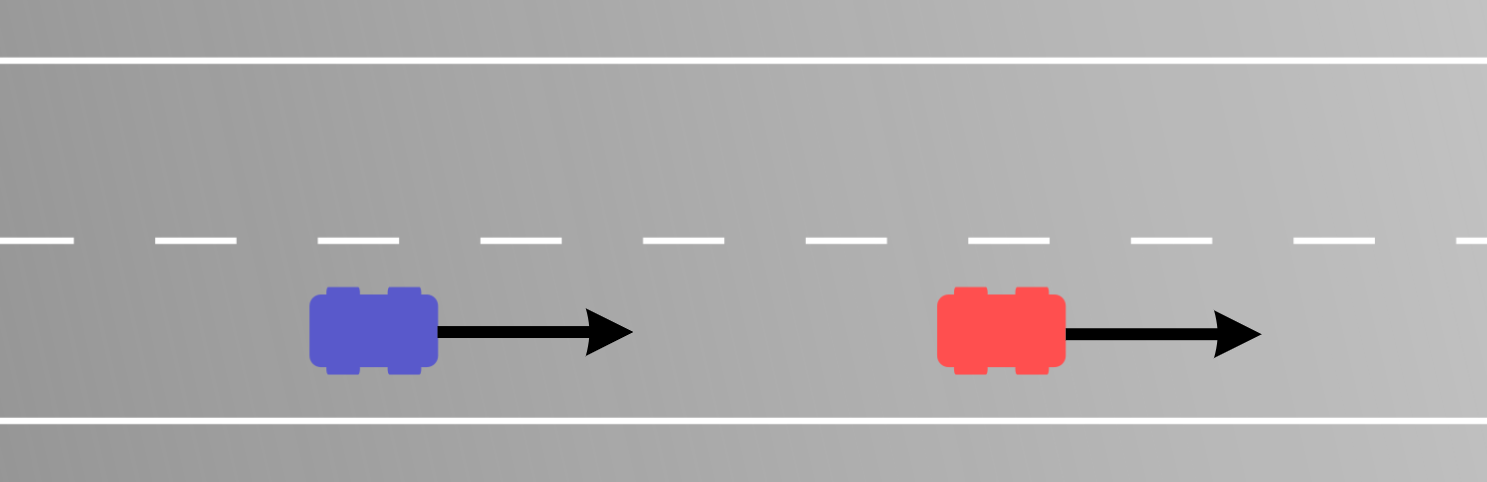
\includegraphics[width=0.48\textwidth]{pics/auto2.png}
  \put(-155,33){\large $\vv{v_1}$}
  \put(-55,33){\large $\vv{v_2}$}
  \put(-190,88){скорости равны $\vv{v_1}=\vv{v_2}$}\hspace*{7mm}
  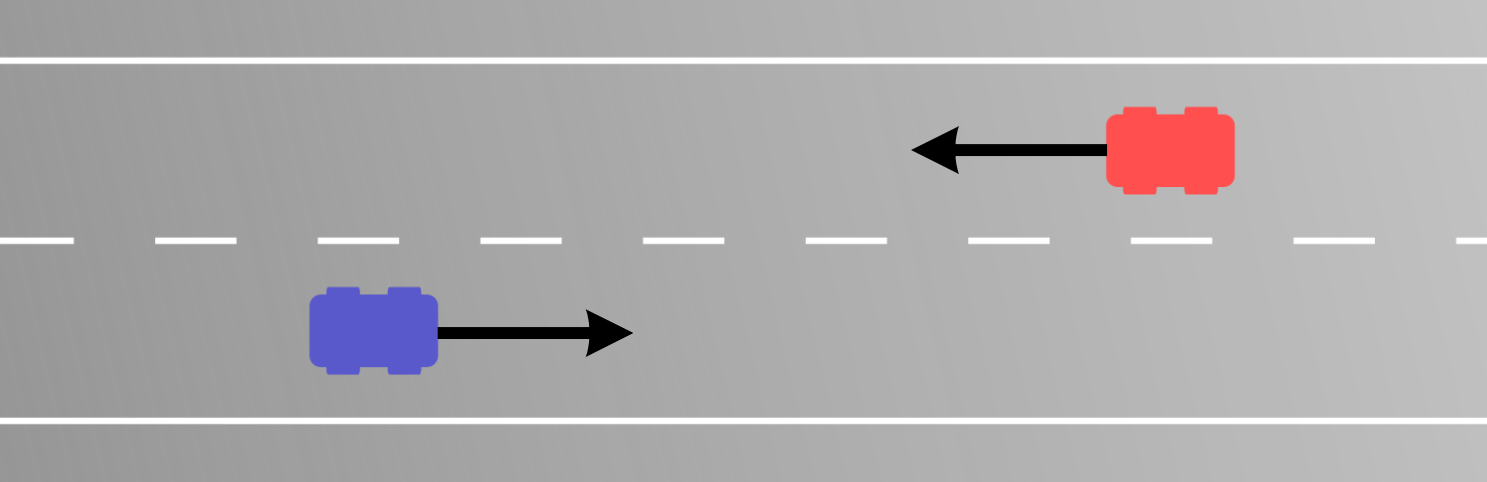
\includegraphics[width=0.48\textwidth]{pics/auto3.png}
  \put(-155,33){\large $\vv{v_1}$}
  \put(-85,65){\large $\vv{v_2}$}
  \put(-220,88){скорости противоположны $\vv{v_1}=-\vv{v_2}$}
  \caption{\small Сонаправленные, противоположно направленные, равные и
  противоположные скорости автомобилей.}\label{pic:auto}
\end{figure}
